\pdfminorversion=4
\documentclass[aspectratio=169]{beamer}

\mode<presentation>
{
  \usetheme{default}
  \usecolortheme{default}
  \usefonttheme{default}
  \setbeamertemplate{navigation symbols}{}
  \setbeamertemplate{caption}[numbered]
  \setbeamertemplate{footline}[frame number]  % or "page number"
  \setbeamercolor{frametitle}{fg=white}
  \setbeamercolor{footline}{fg=black}
} 

\usepackage[english]{babel}
\usepackage{inputenc}
\usepackage{tikz}
\usepackage{courier}
\usepackage{array}
\usepackage{bold-extra}
\usepackage{minted}
\usepackage[thicklines]{cancel}
\usepackage{fancyvrb}
\usepackage{ulem}

\xdefinecolor{dianablue}{rgb}{0.18,0.24,0.31}
\xdefinecolor{darkblue}{rgb}{0.1,0.1,0.7}
\xdefinecolor{darkgreen}{rgb}{0,0.5,0}
\xdefinecolor{darkgrey}{rgb}{0.35,0.35,0.35}
\xdefinecolor{darkorange}{rgb}{0.8,0.5,0}
\xdefinecolor{darkred}{rgb}{0.7,0,0}
\definecolor{darkgreen}{rgb}{0,0.6,0}
\definecolor{mauve}{rgb}{0.58,0,0.82}

\title[2024-01-29-hsf-training-intro]{Last week I wasn't prepared, but today I have slides! \\ \vspace{0.25 cm}\large (Not the same thing\ldots)}
\author{Jim Pivarski}
\institute{Princeton University -- IRIS-HEP}
\date{January 29, 2024}

\usetikzlibrary{shapes.callouts}

\begin{document}

\logo{\pgfputat{\pgfxy(0.11, 7.4)}{\pgfbox[right,base]{\tikz{\filldraw[fill=dianablue, draw=none] (0 cm, 0 cm) rectangle (50 cm, 1 cm);}\mbox{\hspace{-8 cm}
\includegraphics[height=1 cm]{princeton-logo-long.png}\hspace{0.1 cm}\raisebox{0.1 cm}{
\includegraphics[height=0.8 cm]{iris-hep-logo-long.png}}\hspace{0.1 cm}}}}}

\begin{frame}
  \titlepage
\end{frame}

\logo{\pgfputat{\pgfxy(0.11, 7.4)}{\pgfbox[right,base]{\tikz{\filldraw[fill=dianablue, draw=none] (0 cm, 0 cm) rectangle (50 cm, 1 cm);}\mbox{\hspace{-8 cm}
\includegraphics[height=1 cm]{princeton-logo.png}\hspace{0.1 cm}\raisebox{0.1 cm}{
\includegraphics[height=0.8 cm]{iris-hep-logo.png}}\hspace{0.1 cm}}}}}

% Uncomment these lines for an automatically generated outline.
%\begin{frame}{Outline}
%  \tableofcontents
%\end{frame}

% START START START START START START START START START START START START START

\begin{frame}{Main issues, as I understand them (each on its own page)}
\large
\vspace{0.5 cm}
\begin{enumerate}\setlength{\itemsep}{0.35 cm}
\item Online ``Analysis \sout{Preservation} Pipelines'' Training, February 26--29.
\item Go live with the new Training Center website [\href{https://github.com/hsf-training/training-center}{\textcolor{blue}{repo}}, \href{https://hepsoftwarefoundation.org/training/center.html}{\textcolor{blue}{old}}, \href{https://main--nimble-pothos-1ee962.netlify.app/}{\textcolor{blue}{new}}].
\item Diversify types of events: basics are well-covered, last machine learning course was over 3 years ago.
\item New presenters: perpetual. I liked the pay-to-teach idea, and I'm willing to look for grants to implement that.
\item Maintaining material: perpetual. Is this coupled with Software Carpentry subscription?
\item Communication: HSF Training Slack is fine for events, but maybe switch to IRIS-HEP Slack (paid) for preparation?
\end{enumerate}
\end{frame}

\begin{frame}{Online ``Analysis \sout{Preservation} Pipelines'' Training, February 26--29}
\vspace{0.5 cm}
\begin{itemize}\setlength{\itemsep}{0.2 cm}
\item \textcolor{darkblue}{Michel}: Docker training, Docker $\to$ Podman and removing dependence on CI/CD.
\item \textcolor{darkblue}{Marco}: Apptainer (Singularity) training, removing dependence on CI/CD.
\item \textcolor{darkblue}{Andres}: CI/CD GitHub training, removing dependence on containerization.
\item \textcolor{darkblue}{Richa}: CI/CD GitLab training, removing dependence on containerization.
\item \textcolor{darkblue}{Michael}: reviewing all changes.
\item \textcolor{darkblue}{Jim}: setting up Indico/Zoom, scheduling sessions, making announcements.
\item Record new videos live at the event (unless anyone wants to do it beforehand), lightly edit, and link to the updated materials.
\end{itemize}
\end{frame}

\begin{frame}{Go live with the new Training Center website!}
\vspace{0.25 cm}
\begin{columns}
\column{0.55\linewidth}
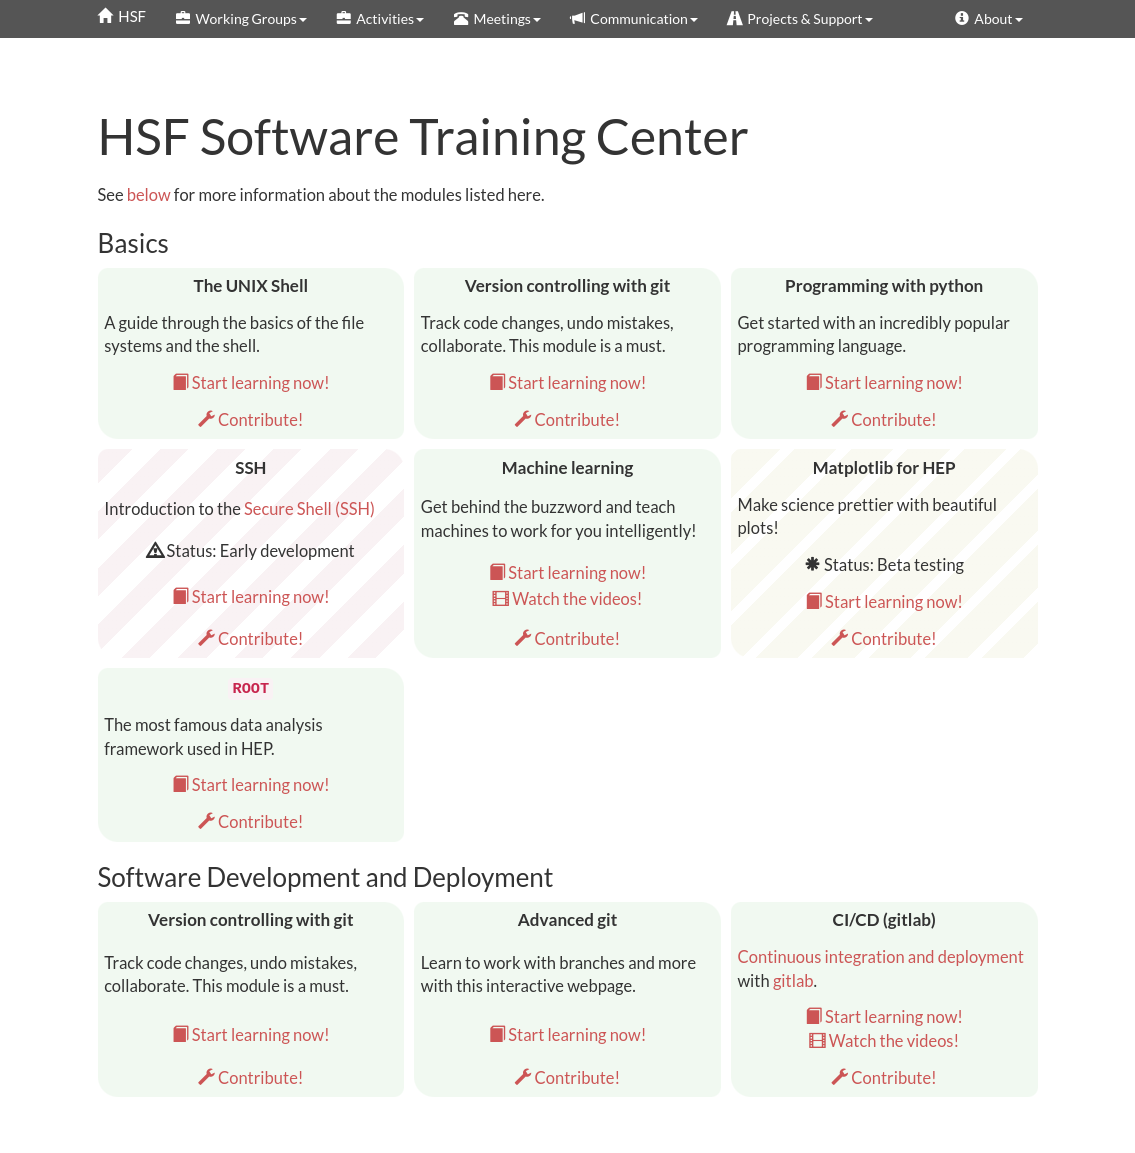
\includegraphics[width=\linewidth]{old-website.png}

\column{0.55\linewidth}
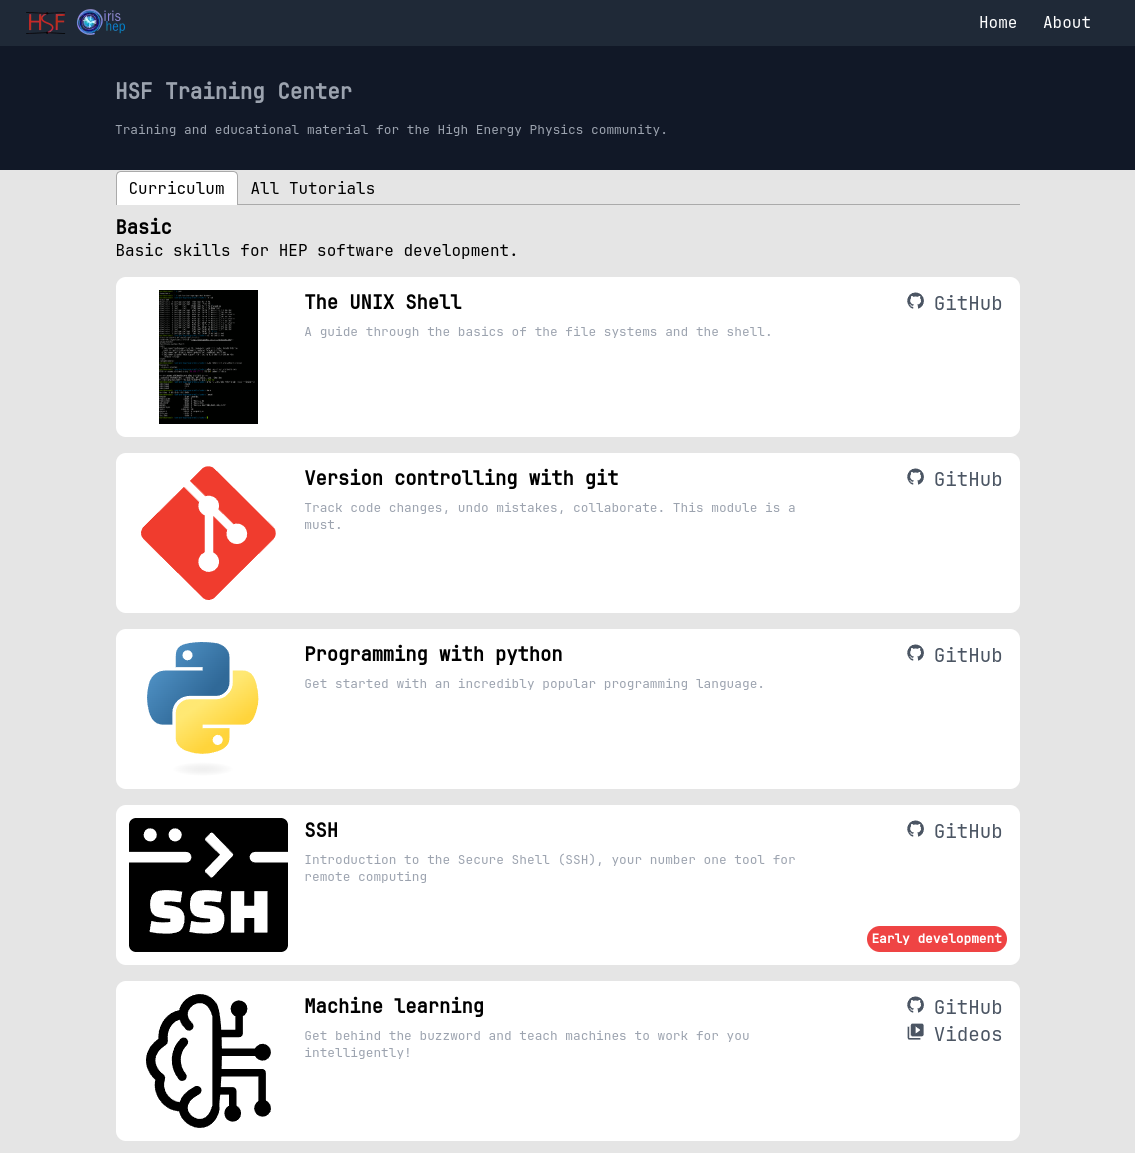
\includegraphics[width=\linewidth]{new-website.png}
\end{columns}
\end{frame}

\begin{frame}{Diversify types of events}
\vspace{0.2 cm}
\begin{columns}[t]
\column{0.55\linewidth}
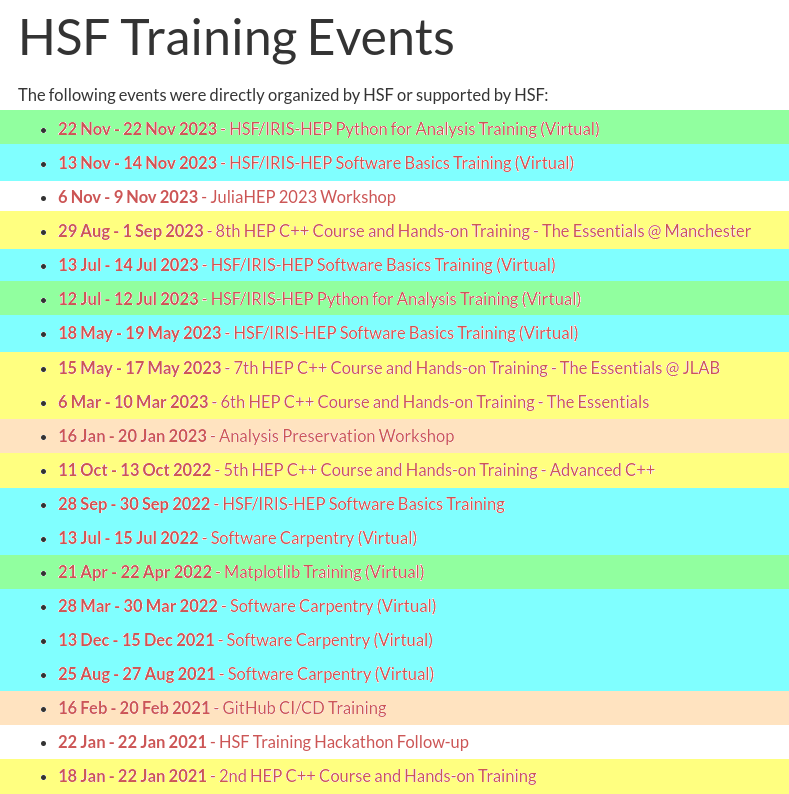
\includegraphics[width=\linewidth]{training-3years.png}

\column{0.55\linewidth}
\only<1>{
\includegraphics[width=\linewidth]{all-offerings.png}}\only<2->{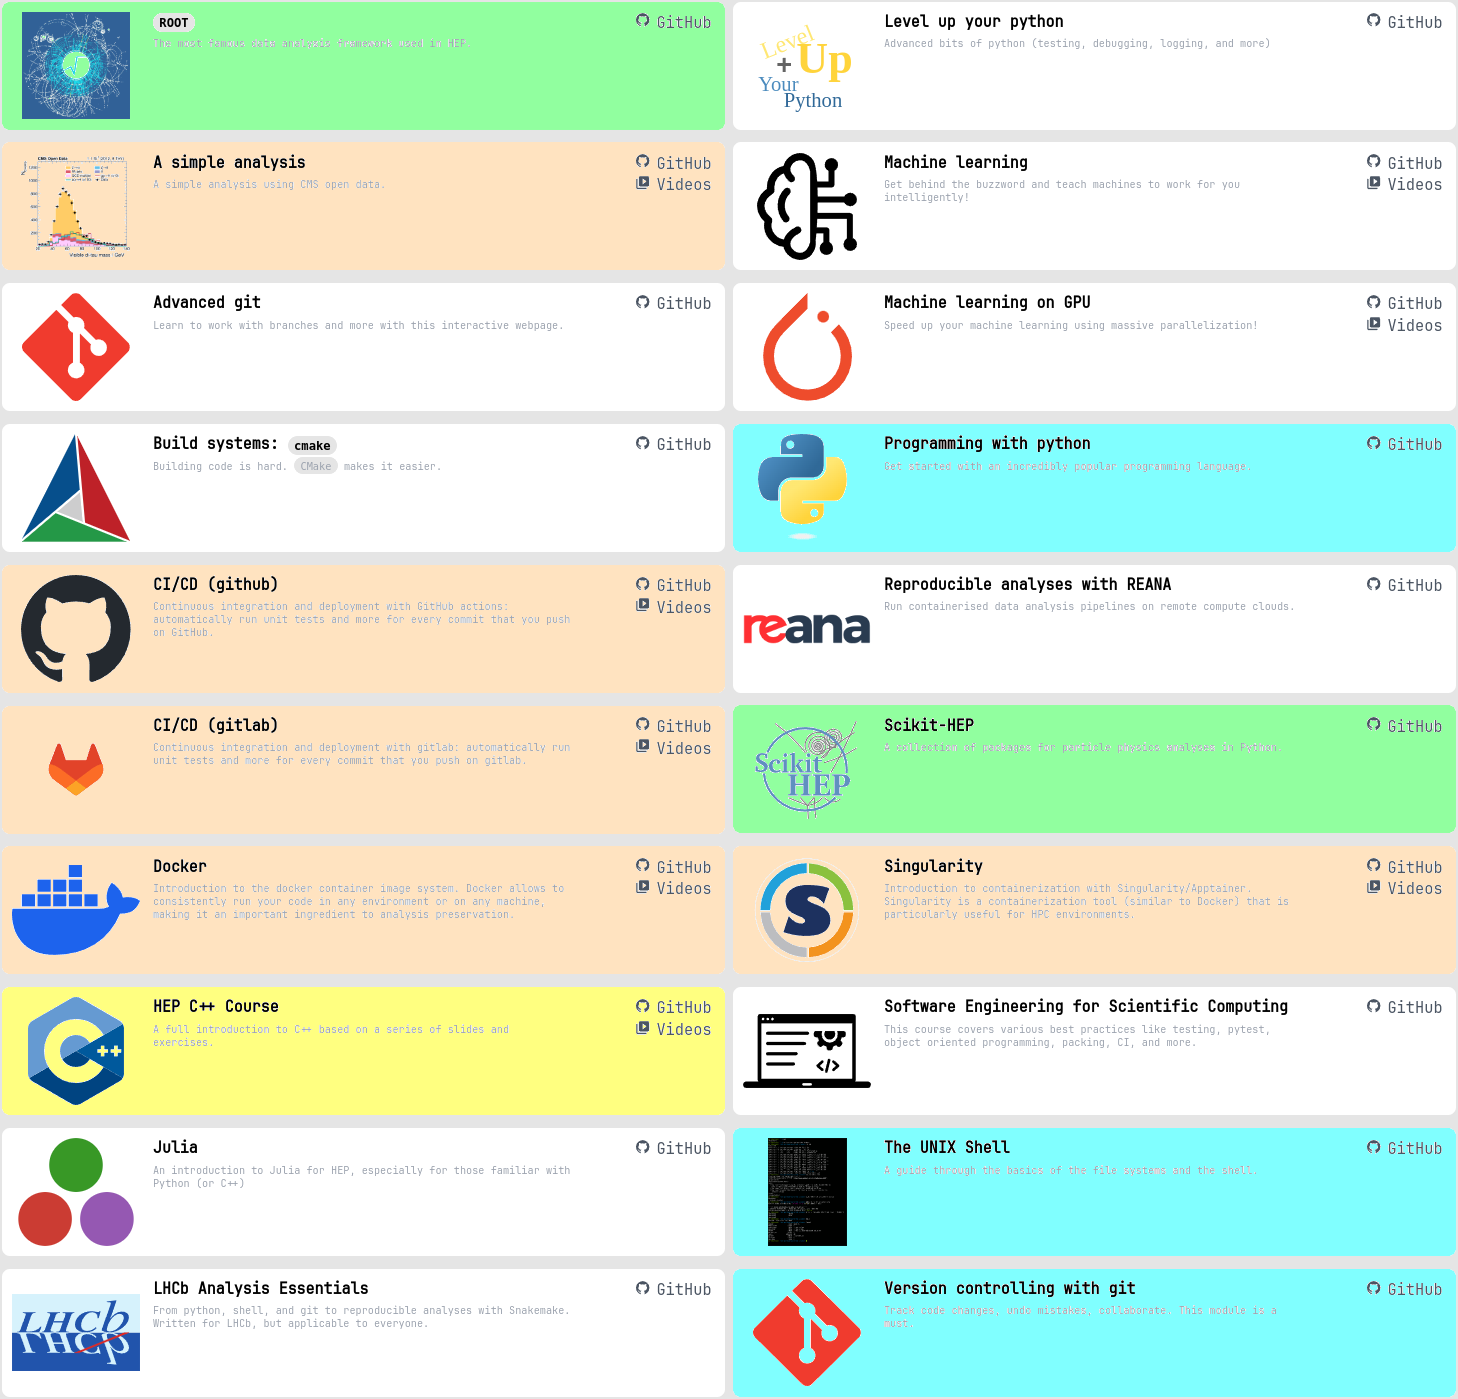
\includegraphics[width=\linewidth]{all-offerings-2.png}}

\begin{center}
\vspace{-7.25 cm}
\uncover<3->{\only<3>{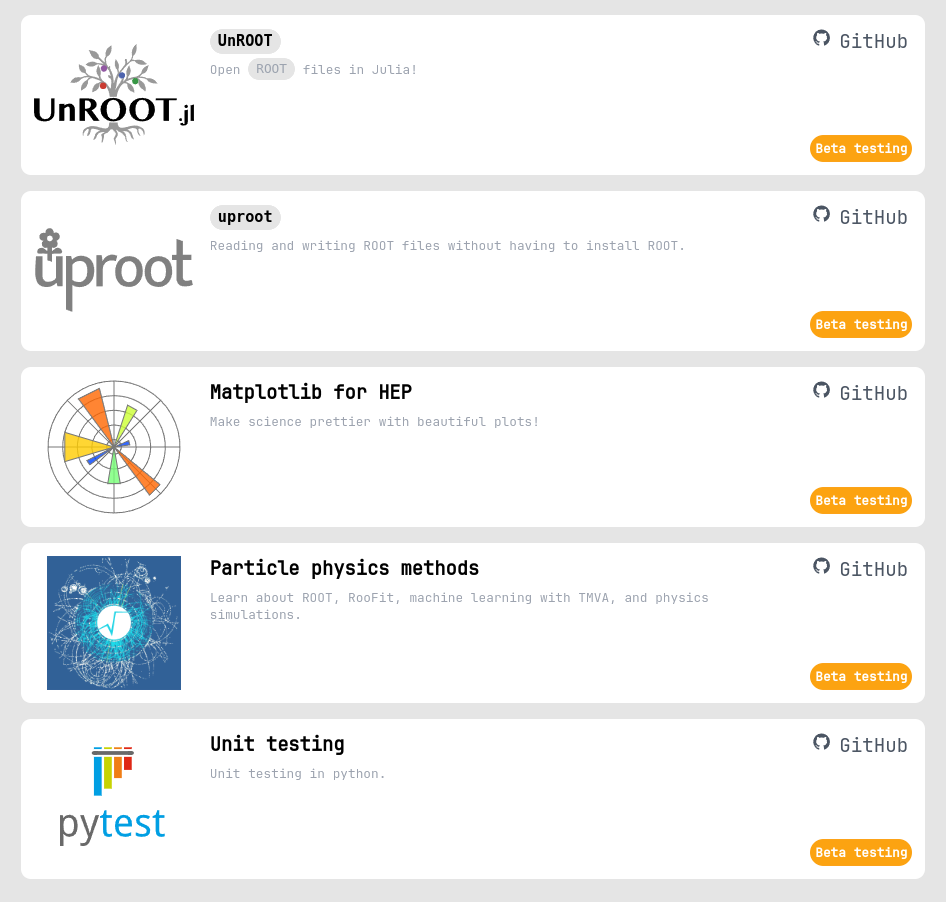
\includegraphics[width=0.9\linewidth]{all-offerings-3.png}}\only<4>{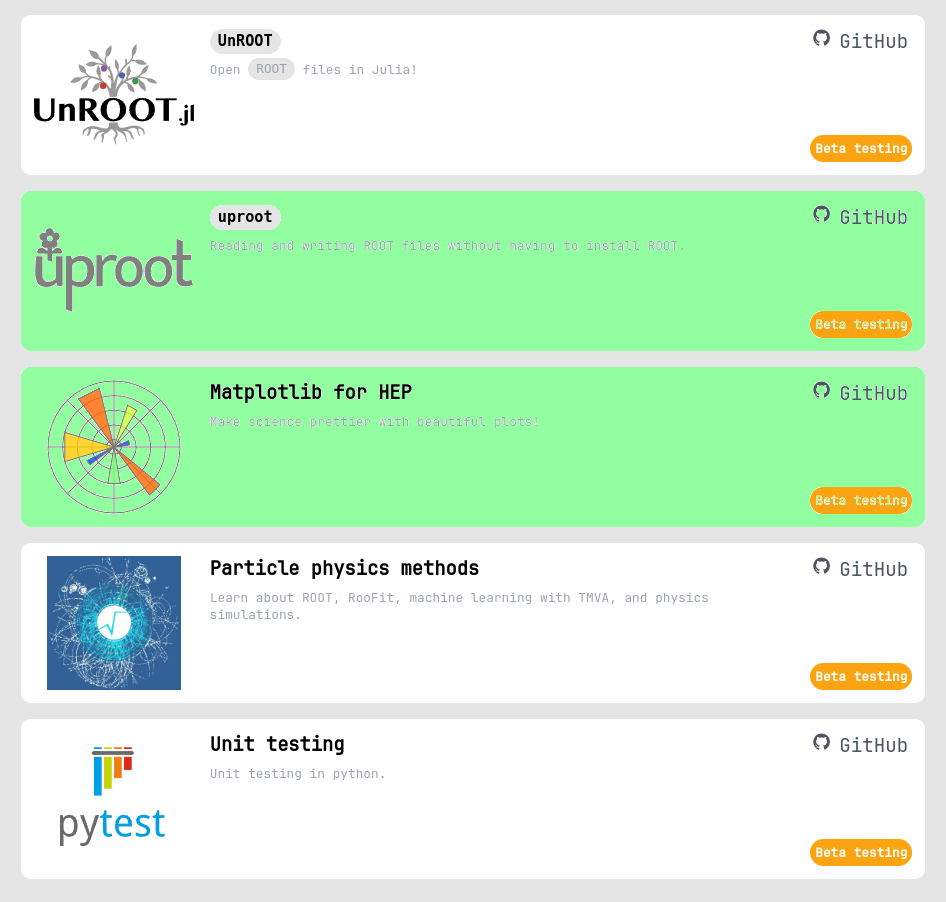
\includegraphics[width=0.9\linewidth]{all-offerings-4.png}}}
\vspace{7.25 cm}
\end{center}

\end{columns}
\end{frame}

\begin{frame}{New presenters: perpetual}
\vspace{0.5 cm}
I liked the pay-to-teach idea, and I'm willing to look for grants to implement that.

\vspace{1 cm}
What was wrong with it? Why was it killed?
\end{frame}

\begin{frame}{Maintaining material: perpetual.}
\vspace{0.5 cm}
\begin{itemize}\setlength{\itemsep}{0.2 cm}
\item Content can get out of date: \href{https://github.com/hsf-training/hsf-training-scikit-hep-webpage/pull/64}{\textcolor{blue}{hsf-training/hsf-training-scikit-hep-webpage\#64}}.
\item In the Awkward Array project, we use \href{https://jupyterbook.org/}{\textcolor{blue}{JupyterBook}} to generate documentation so that \href{https://github.com/scikit-hep/awkward/actions/workflows/docs.yml}{\textcolor{blue}{it can be tested}} (and deployed) in each PR.
\begin{center}

\includegraphics[width=0.75\linewidth]{view-deployment.png}
\end{center}
\item We're currently using a Jekyll template from Software Carpentry that's no longer the one they're maintaining.
\item If we have to transfer markdown anyway, perhaps we should go to Jupyter?
\item Consider, for low-dependency tutorials: \textcolor{blue}{\small\url{https://jupyter.org/try-jupyter/}}
\end{itemize}

\vspace{0.25 cm}
\small
Used successfully at CoDaS-HEP: \textcolor{blue}{\url{https://ioanaif.github.io/columnar-data-analysis-codas-hep-2023/}}
\end{frame}

\begin{frame}{Communication: switch to IRIS-HEP Slack (paid) for preparation?}
\vspace{0.35 cm}
\begin{columns}
\column{1.1\linewidth}
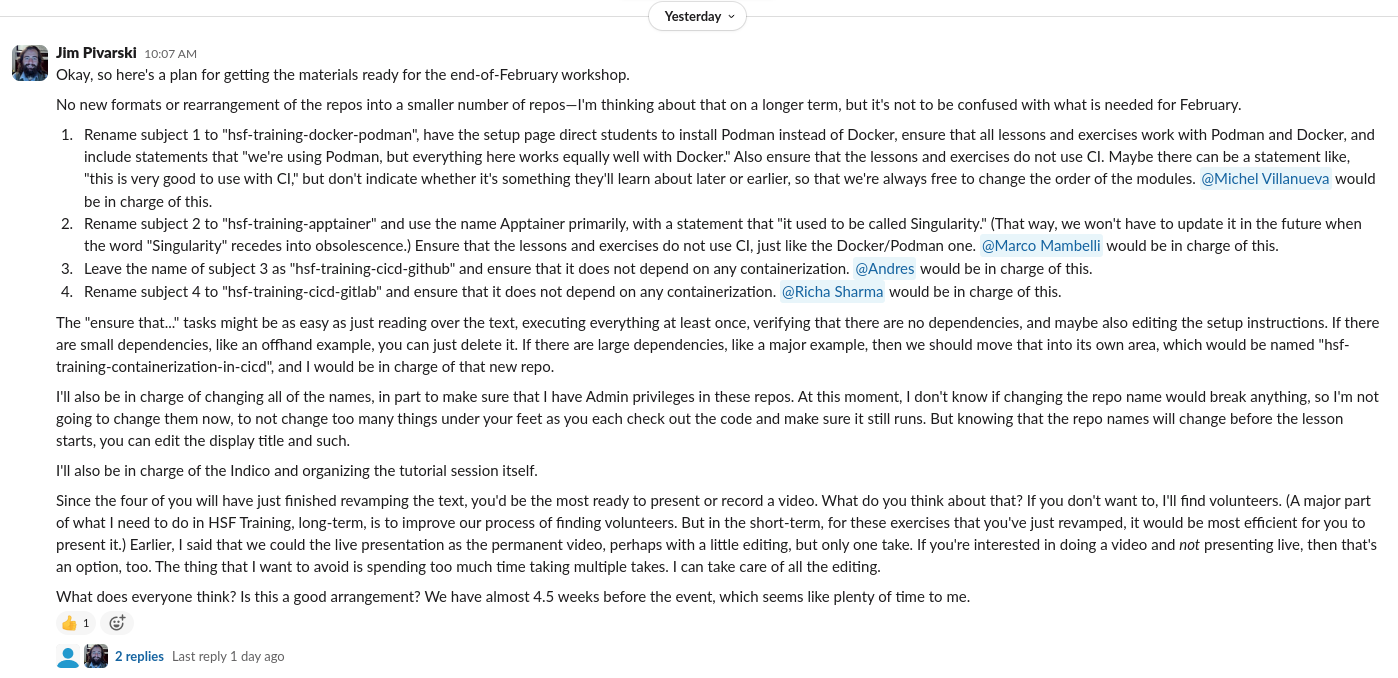
\includegraphics[width=\linewidth]{big-slack-comments.png}
\end{columns}
\end{frame}

\end{document}
